\begin{itemize}
    \color{red}
    \item focus on track finding and fitting performance
    \item mention+cite CTD contribution, what is the difference to today?
    \item how do we measure the performance
    \begin{itemize}
        \item simulation, params, cuts
        \item reconstruction chain, params, cuts
        \item aggregation of the performance metrics
    \end{itemize}
    \item what are the limitations of performance studies with ACTS Examples?
    \item pre conditions
    \begin{itemize}
        \item material mapping
        \item magnetic field
        \item alignment
        \item fast digitization - for digital we do not need any plots, for geometric it would be good
    \end{itemize}
\end{itemize}

\section{Simulation}

\begin{itemize}
    \color{red}
    \item event generation: particle gun / Pythia8
    \item detector simulation: Fatras / Geant4
    \item digitization: truth based, smeared / geometric
\end{itemize}

\section{Clustering}

\begin{itemize}
    \item truth based
    \item in case of geometric, show residuals and pulls, potentially per cluster size
\end{itemize}

\section{Seeding}

\begin{itemize}
    \color{red}
    \item configuration not optimized, not the focus of this thesis
    \item explain different seeding algorithms?
    \item show seeding configuration?
    \item show the performance of the default seeding algorithm compared to the truth one
    \begin{itemize}
        \item efficiency
        \item fake rate
        \item purity
        \item initial parameter residuals?
    \end{itemize}
    \item above metrics as a function of
    \begin{itemize}
        \item pileup
        \item eta, phi, pt
    \end{itemize}
\end{itemize}

\begin{figure}[h]
    \centering
    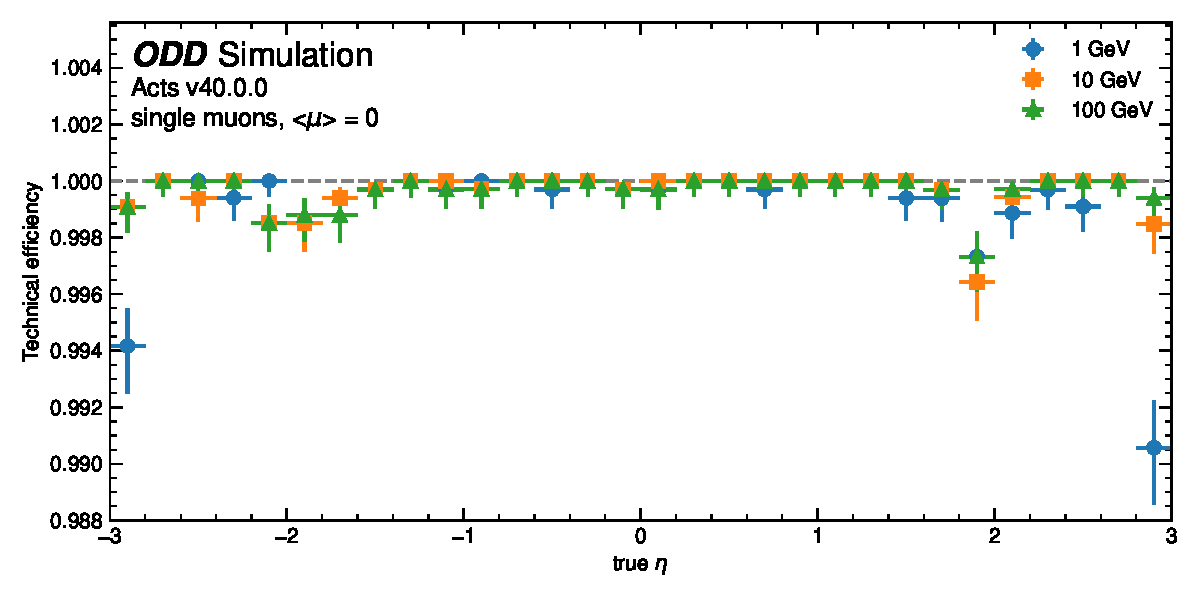
\includegraphics[width=1.0\textwidth]{parts/3_performance/11_acts-performance/figures/seeding_efficiency_mu.pdf}
    \caption{Seeding efficiency as a function of eta for single muons with 1, 10, 100 GeV transverse momentum.}
    \label{fig:perf/odd/seeding-efficiency-mu}
\end{figure}

\begin{figure}[h]
    \centering
    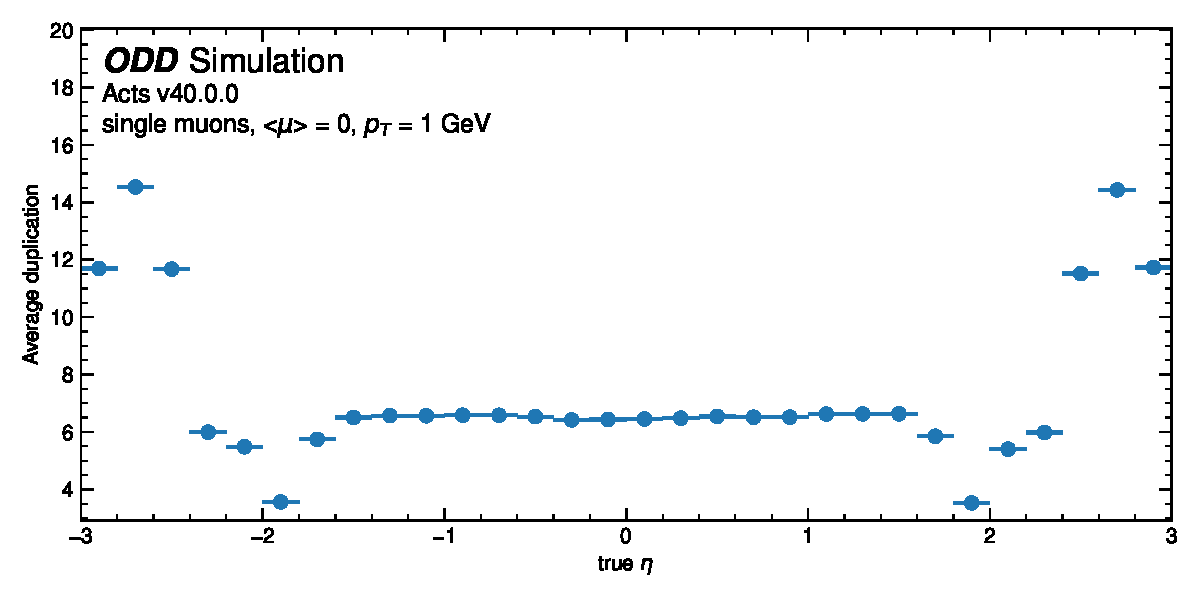
\includegraphics[width=1.0\textwidth]{parts/3_performance/11_acts-performance/figures/seeding_duplication.pdf}
    \caption{Seed duplication as a function of eta for single muons with 1 GeV transverse momentum.}
    \label{fig:perf/odd/seeding-duplication}
\end{figure}

\begin{figure}[h]
    \centering
    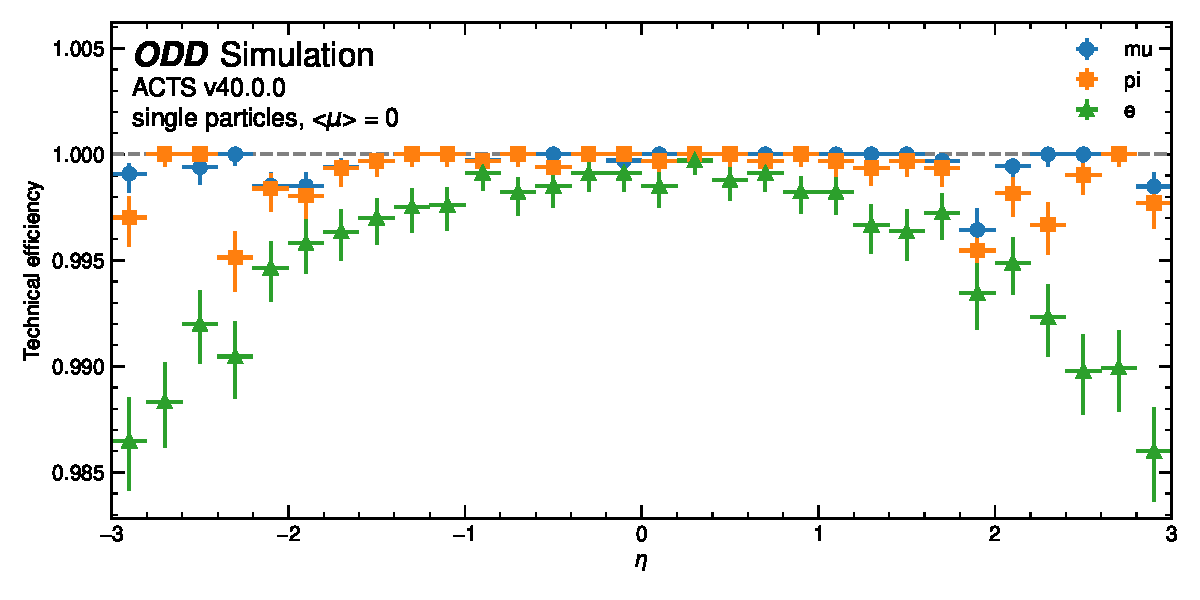
\includegraphics[width=1.0\textwidth]{parts/3_performance/11_acts-performance/figures/seeding_efficiency_mixed.pdf}
    \caption{Seeding efficiency as a function of eta for single muons, pions, and electrons with 10 GeV transverse momentum.}
    \label{fig:perf/odd/seeding-efficiency-mixed}
\end{figure}

\begin{figure}[h]
    \centering
    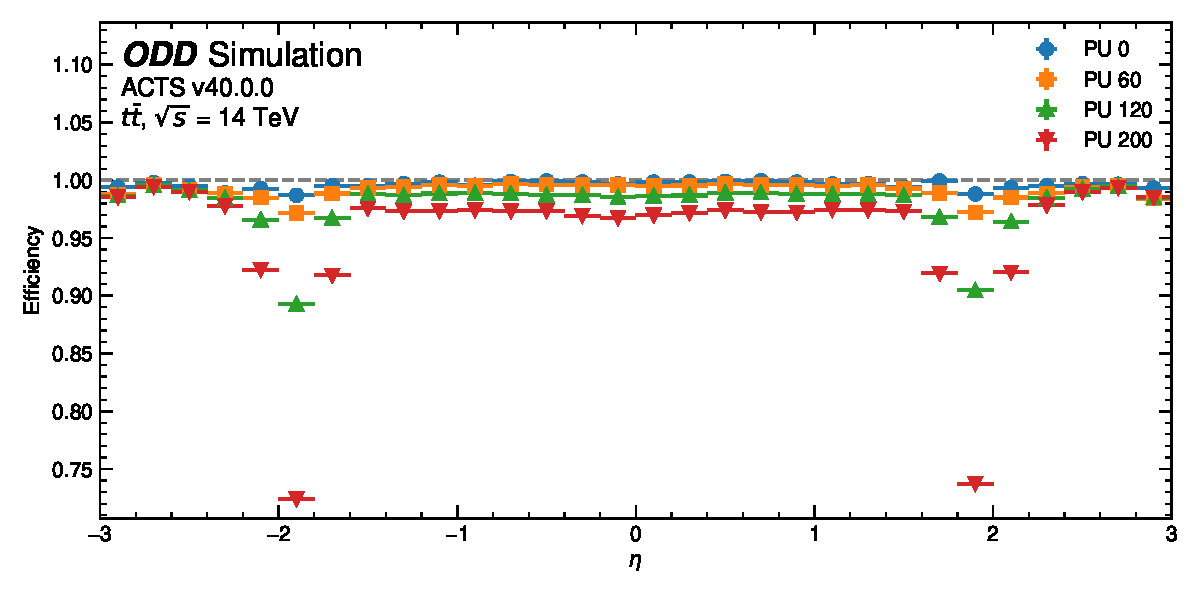
\includegraphics[width=1.0\textwidth]{parts/3_performance/11_acts-performance/figures/seeding_efficiency_ttbar.pdf}
    \caption{Seeding efficiency as a function of eta for \ttbar events with different pileup.}
    \label{fig:perf/odd/seeding-efficiency-ttbar}
\end{figure}

\begin{figure}[h]
    \centering
    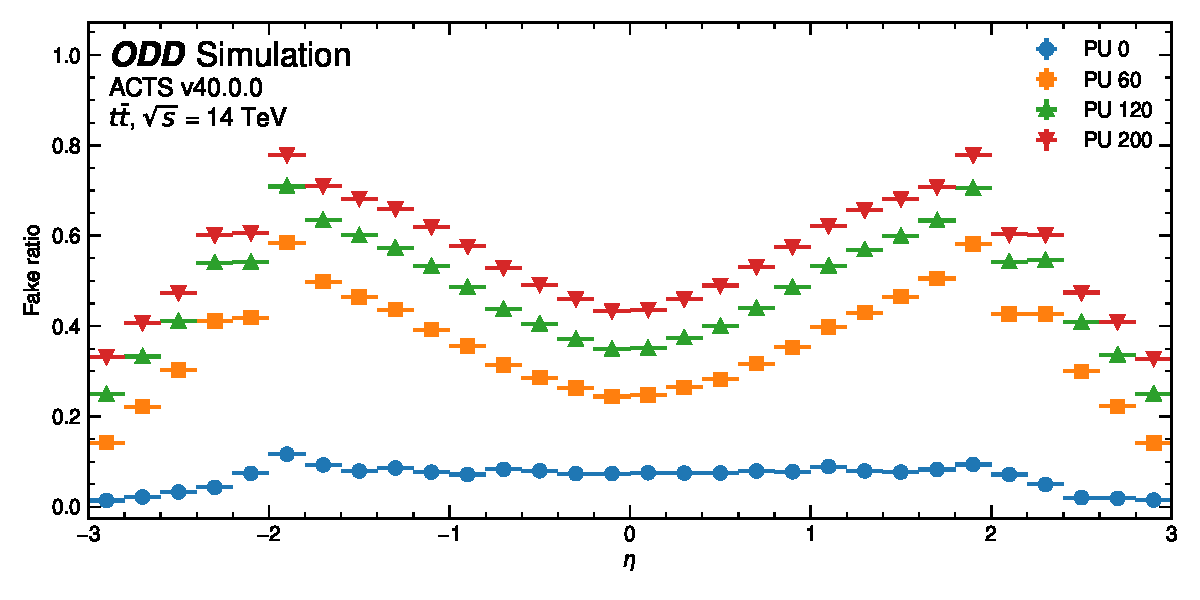
\includegraphics[width=1.0\textwidth]{parts/3_performance/11_acts-performance/figures/seeding_fake_ttbar.pdf}
    \caption{Seeding fake ratio as a function of eta for \ttbar events with different pileup.}
    \label{fig:perf/odd/seeding-fake-ttbar}
\end{figure}

\section{Combinatorial Kalman Filter}

\begin{itemize}
    \color{red}
    \item explain the CKF algorithm
    \item show the performance of the CKF compared to the seeding
    \begin{itemize}
        \item efficiency
        \item n duplicates
        \item fake rate
        \item purity?
        \item initial parameter residuals
    \end{itemize}
    \item above metrics as a function of
    \begin{itemize}
        \item pileup
        \item eta, phi, pt
    \end{itemize}
\end{itemize}

\begin{figure}[h]
    \centering
    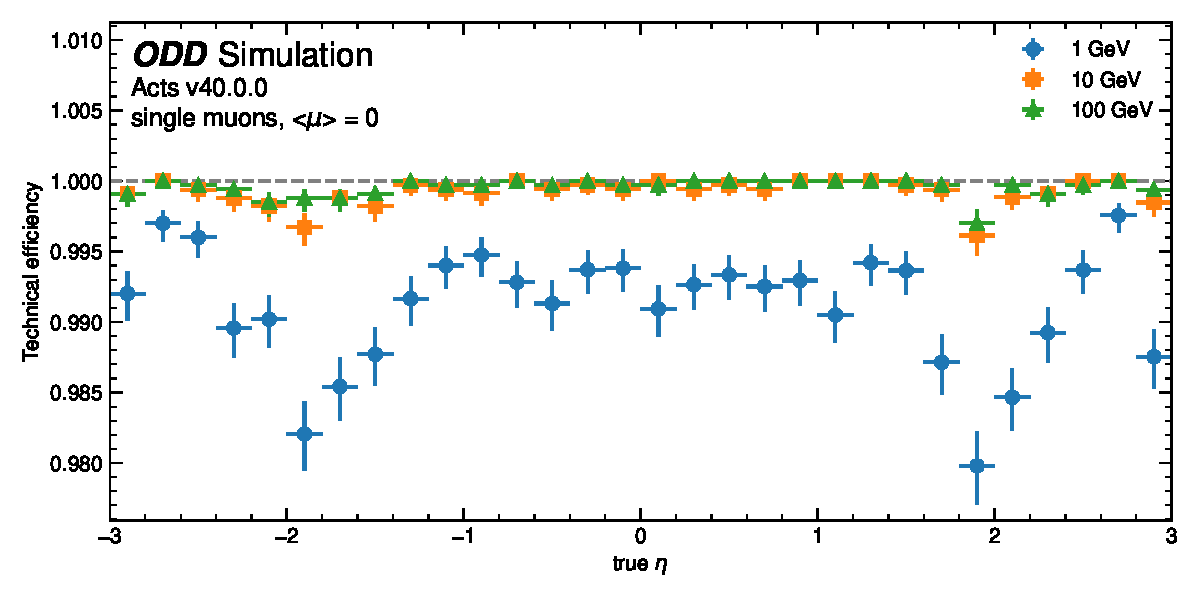
\includegraphics[width=1.0\textwidth]{parts/3_performance/11_acts-performance/figures/finding_efficiency_mu.pdf}
    \caption{Finding efficiency as a function of eta for single muons with 1, 10, 100 GeV transverse momentum.}
    \label{fig:perf/odd/finding-efficiency-mu}
\end{figure}

\begin{figure}[h]
    \centering
    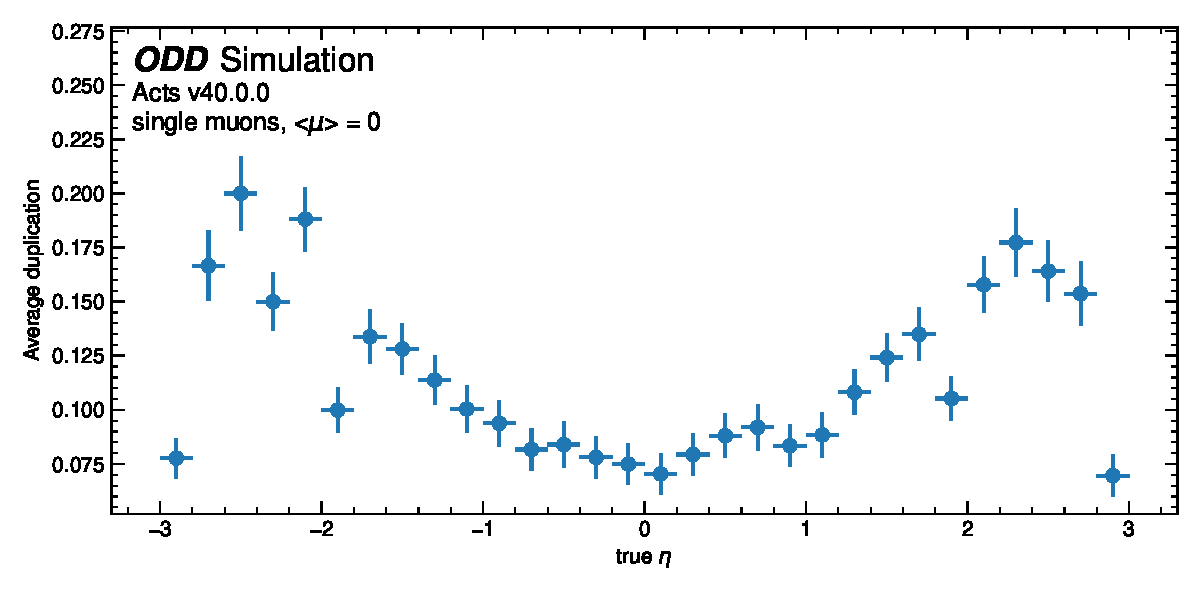
\includegraphics[width=1.0\textwidth]{parts/3_performance/11_acts-performance/figures/finding_duplication.pdf}
    \caption{Finding duplication as a function of eta for single muons with 1 GeV transverse momentum.}
    \label{fig:perf/odd/finding-duplication}
\end{figure}

\begin{figure}[h]
    \centering
    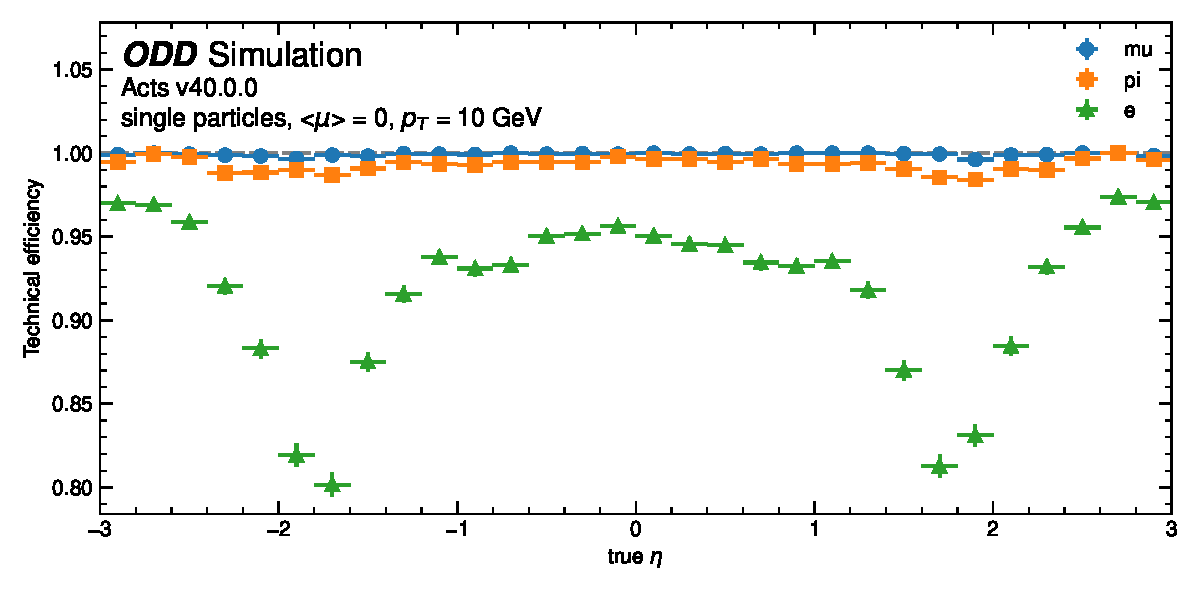
\includegraphics[width=1.0\textwidth]{parts/3_performance/11_acts-performance/figures/finding_efficiency_mixed.pdf}
    \caption{Finding efficiency as a function of eta for single muons, pions, and electrons with 10 GeV transverse momentum.}
    \label{fig:perf/odd/finding-efficiency-mixed}
\end{figure}

\begin{figure}[h]
    \centering
    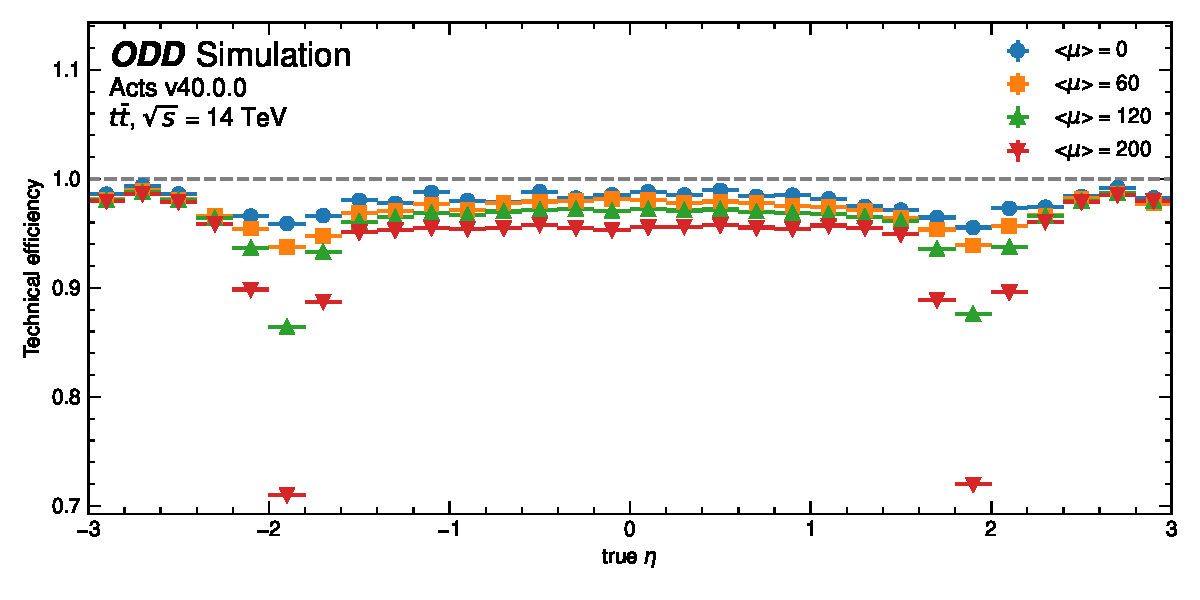
\includegraphics[width=1.0\textwidth]{parts/3_performance/11_acts-performance/figures/finding_efficiency_ttbar.pdf}
    \caption{Finding efficiency as a function of eta for \ttbar events with different pileup.}
    \label{fig:perf/odd/finding-efficiency-ttbar}
\end{figure}

\begin{figure}[h]
    \centering
    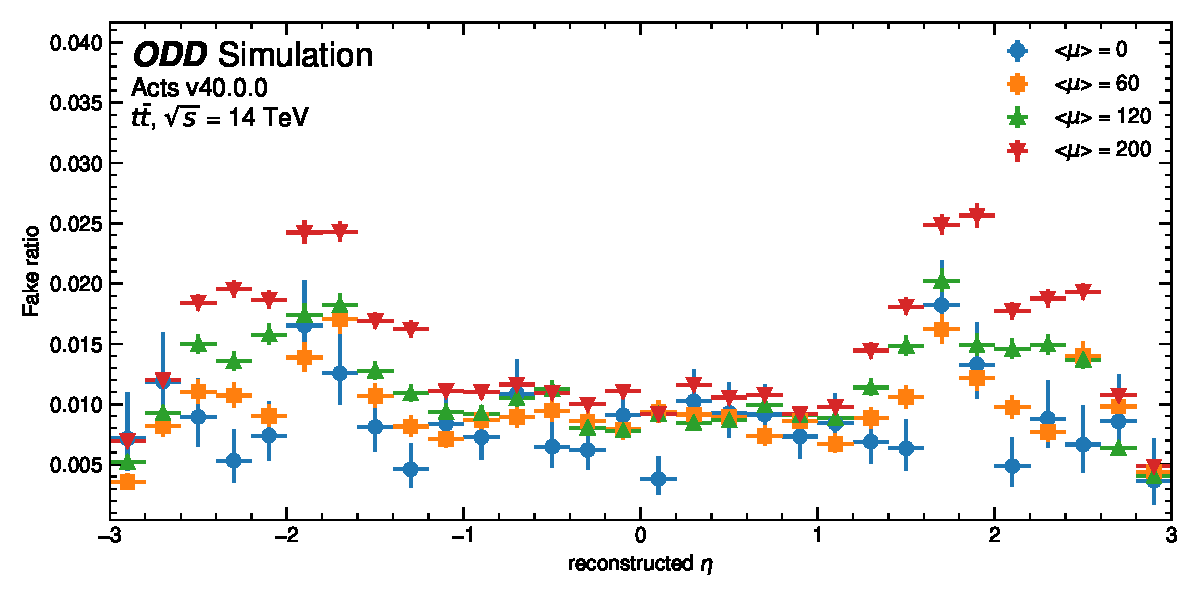
\includegraphics[width=1.0\textwidth]{parts/3_performance/11_acts-performance/figures/finding_fake_ttbar.pdf}
    \caption{Finding fake ratio as a function of eta for \ttbar events with different pileup.}
    \label{fig:perf/odd/finding-fake-ttbar}
\end{figure}

\begin{figure}[h]
    \centering
    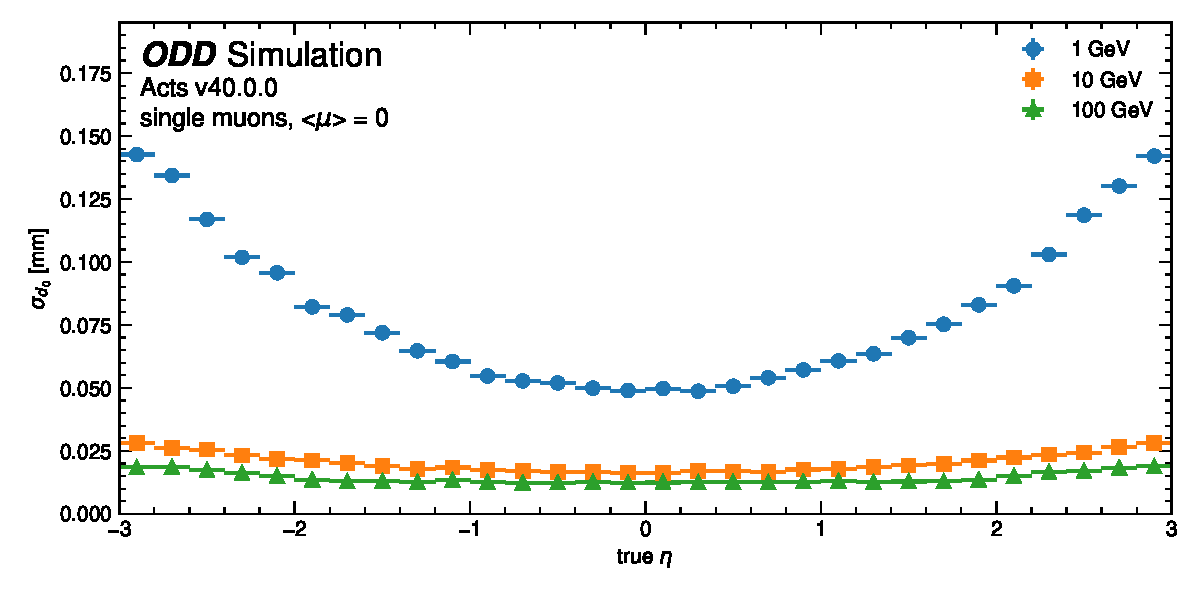
\includegraphics[width=1.0\textwidth]{parts/3_performance/11_acts-performance/figures/fitting_resolution_d0_vs_eta_mu.pdf}
    \caption{}
    \label{fig:perf/odd/fitting-resolution-d0-eta-mu}
\end{figure}

\begin{figure}[h]
    \centering
    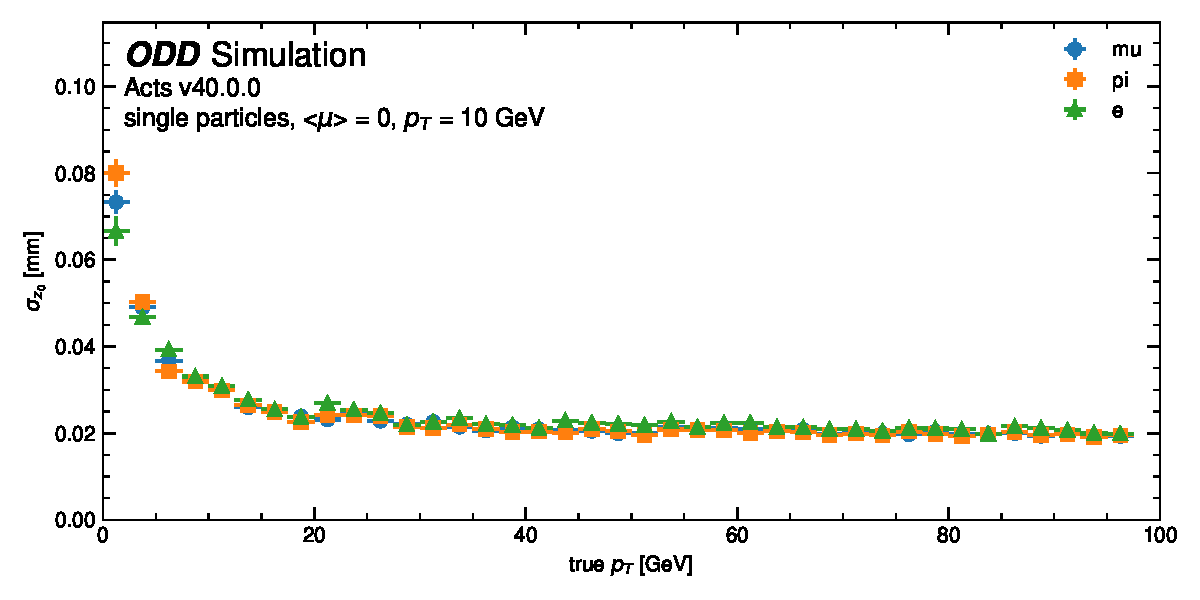
\includegraphics[width=1.0\textwidth]{parts/3_performance/11_acts-performance/figures/fitting_resolution_z0_vs_pt_mixed.pdf}
    \caption{}
    \label{fig:perf/odd/fitting-resolution-z0-pt-mixed}
\end{figure}

\begin{figure}[h]
    \centering
    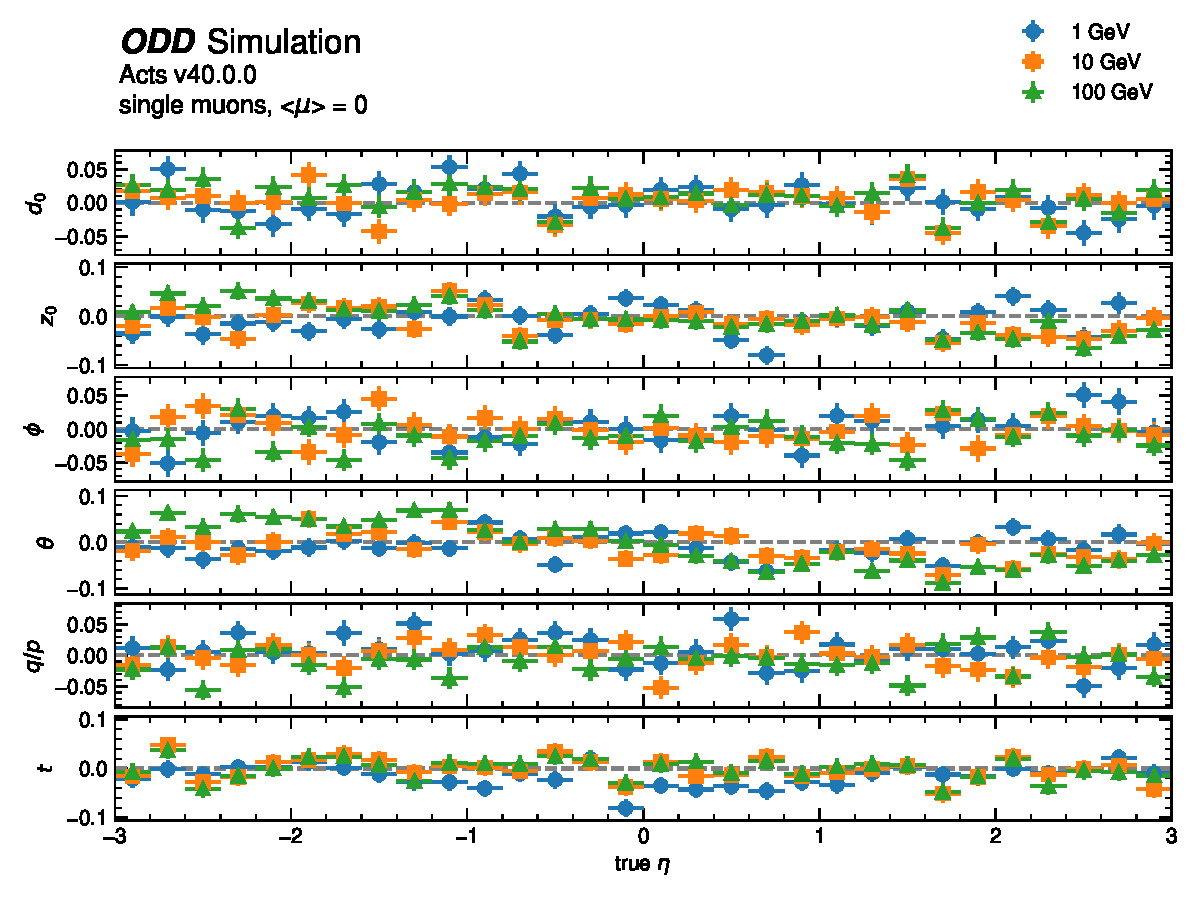
\includegraphics[width=1.0\textwidth]{parts/3_performance/11_acts-performance/figures/fitting_pullmean_vs_eta_mu.pdf}
    \caption{}
    \label{fig:perf/odd/fitting-pullmean-eta-mu}
\end{figure}

\begin{figure}[h]
    \centering
    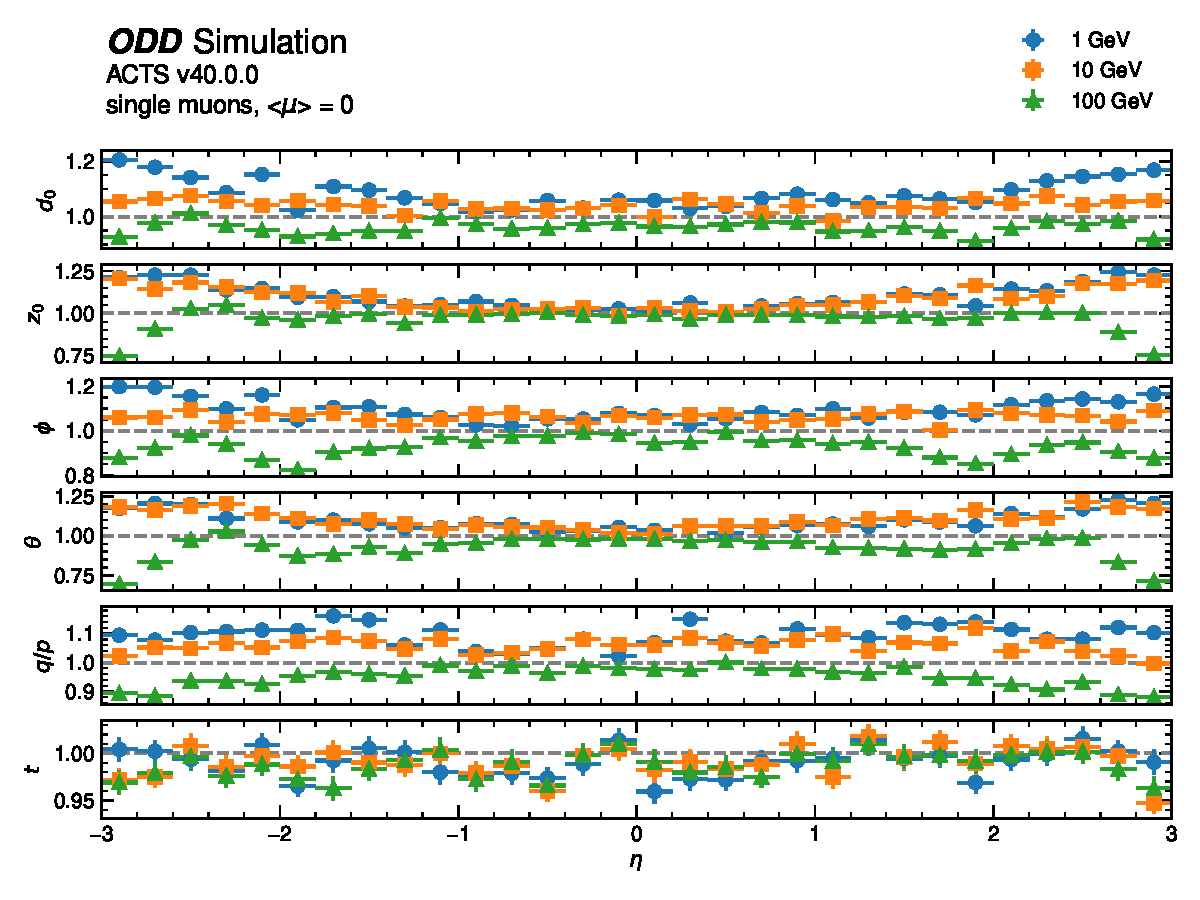
\includegraphics[width=1.0\textwidth]{parts/3_performance/11_acts-performance/figures/fitting_pullwidth_vs_eta_mu.pdf}
    \caption{}
    \label{fig:perf/odd/fitting-pullwidth-eta-mu}
\end{figure}

\section{Ambiguity resolution}

\begin{itemize}
    \color{red}
    \item explain the greedy ambiguity resolution algorithm quickly
    \item link to the impl section
    \item show the performance of the ambiguity resolution compared to the CKF
\end{itemize}

\begin{figure}[h]
    \centering
    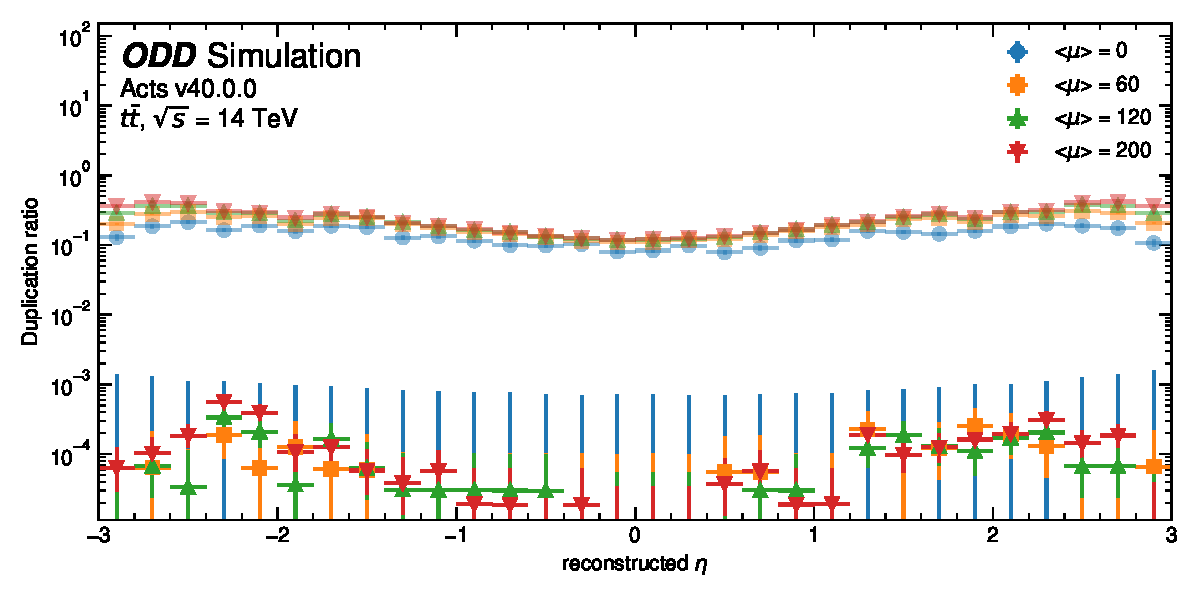
\includegraphics[width=1.0\textwidth]{parts/3_performance/11_acts-performance/figures/ambi_duplication_ttbar.pdf}
    \caption{}
    \label{fig:perf/odd/ambi-duplication-ttbar}
\end{figure}

\section{Track fitting}

\begin{itemize}
    \color{red}
    \item explain the track fitting algorithm
    \item why refit after finding?
    \item IP resolution vs CKF
\end{itemize}

\begin{figure}[h]
    \centering
    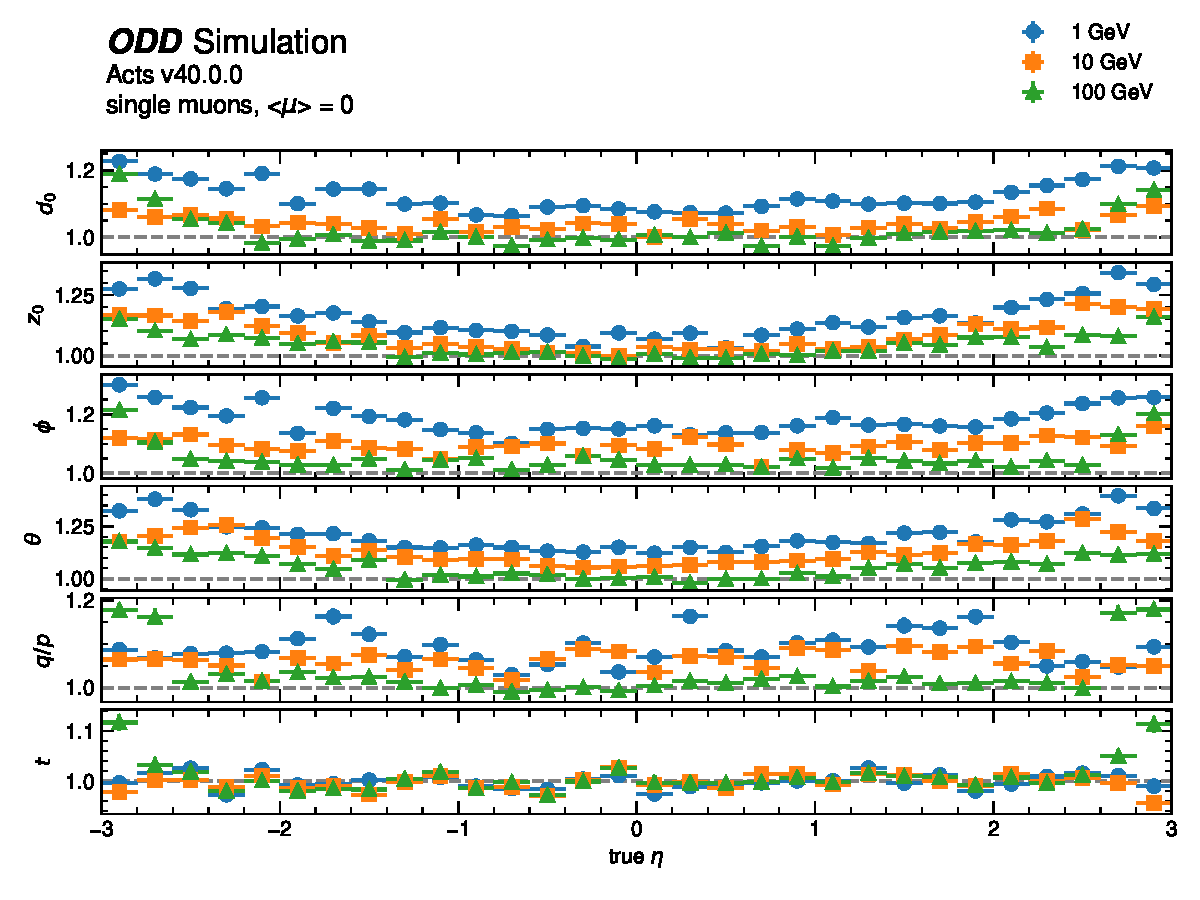
\includegraphics[width=1.0\textwidth]{parts/3_performance/11_acts-performance/figures/refit_pullwidth_vs_eta_mu.pdf}
    \caption{}
    \label{fig:perf/odd/refit-pullwidth-eta-mu}
\end{figure}

\section{Vertexing}

\begin{itemize}
    \color{red}
    \item explain the vertexing algorithm
    \item resolutions and pulls for hard scatter
    \item efficiency, split rate, merge rate vs pileup
    \item 3D vs 4D
\end{itemize}

\begin{figure}[h]
    \centering
    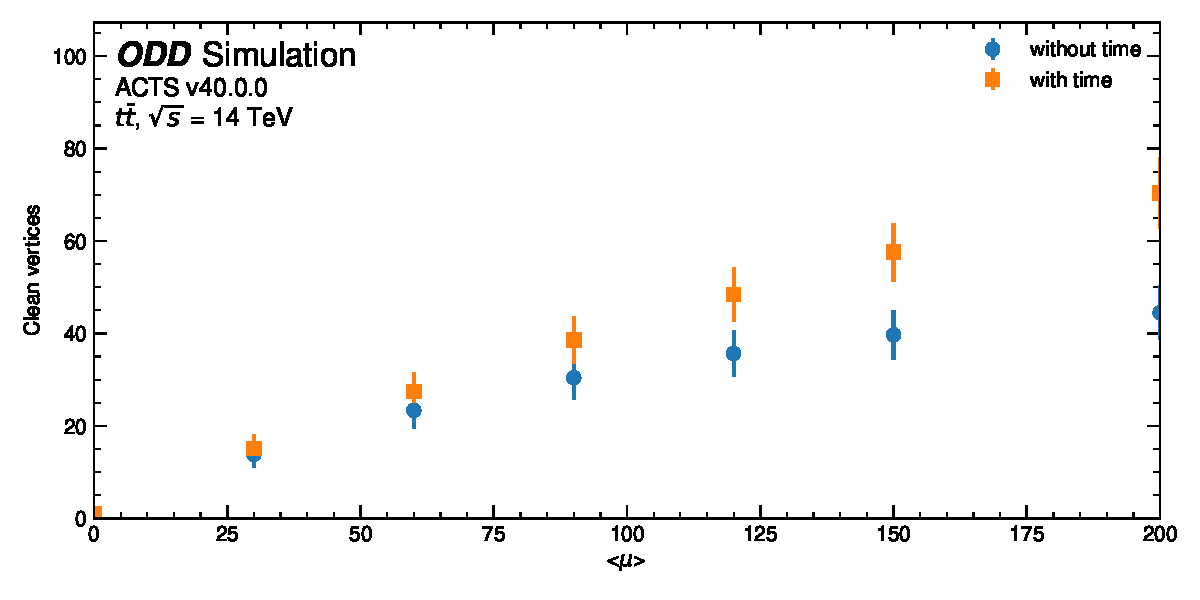
\includegraphics[width=1.0\textwidth]{parts/3_performance/11_acts-performance/figures/vertex_efficiency.pdf}
    \caption{}
    \label{fig:perf/odd/vertex-efficiency}
\end{figure}

\begin{figure}[h]
    \centering
    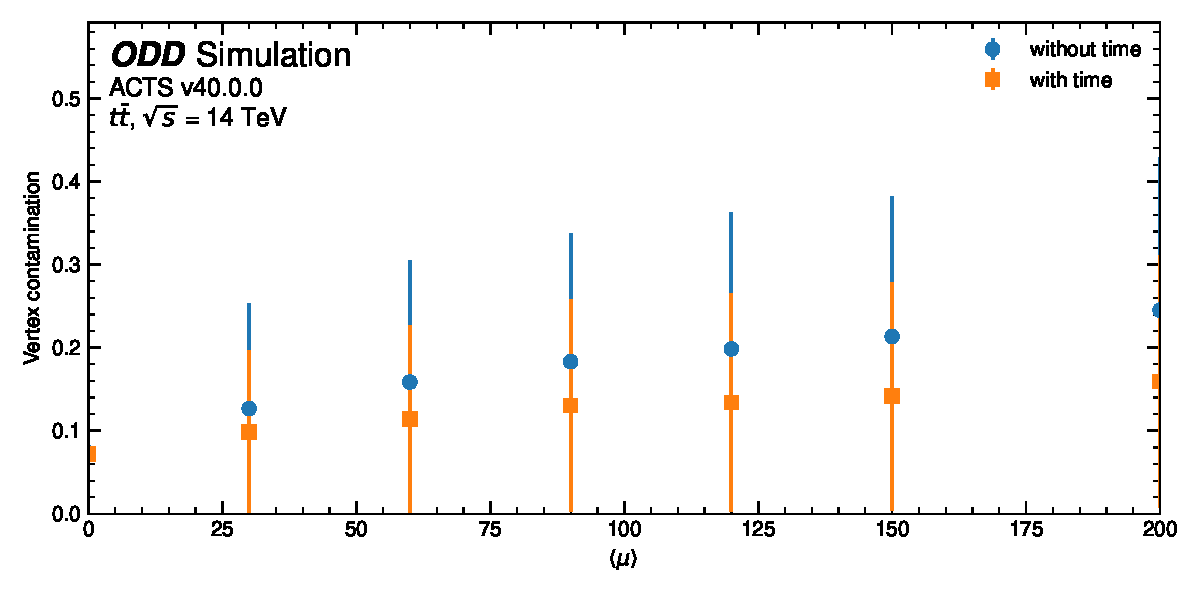
\includegraphics[width=1.0\textwidth]{parts/3_performance/11_acts-performance/figures/vertex_contamination.pdf}
    \caption{}
    \label{fig:perf/odd/vertex-contamination}
\end{figure}

\begin{figure}[h]
    \centering
    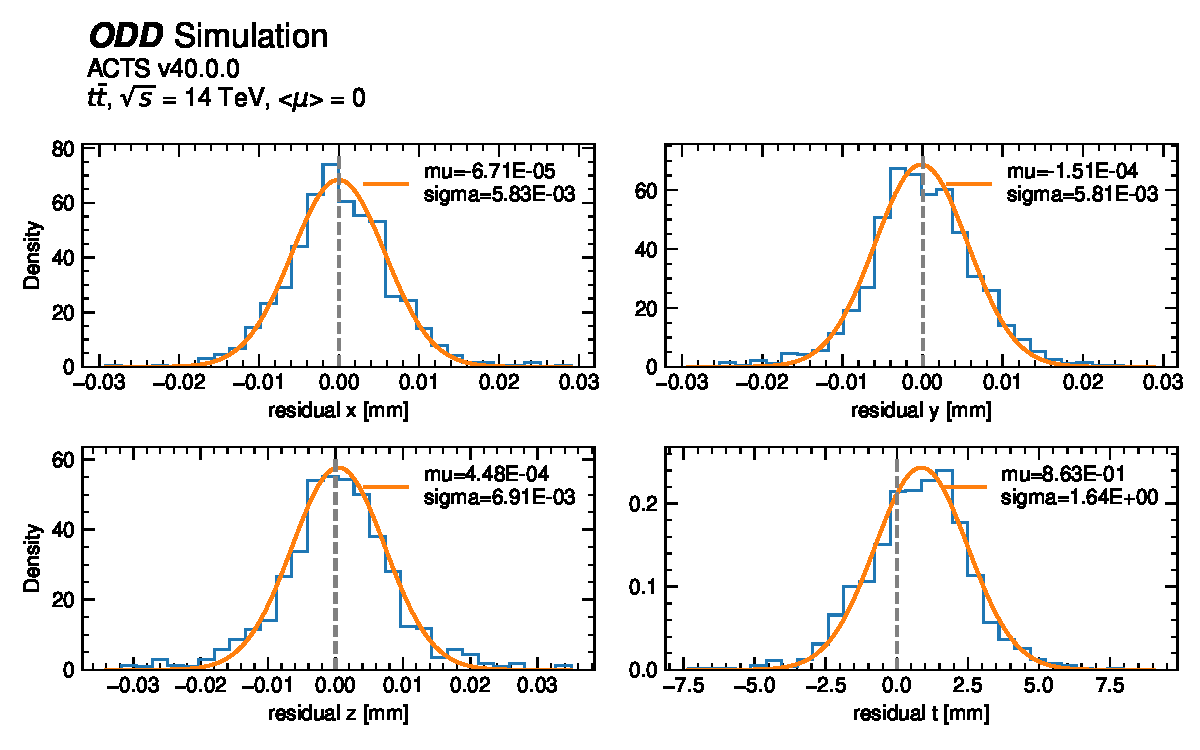
\includegraphics[width=1.0\textwidth]{parts/3_performance/11_acts-performance/figures/vertex_resolution.pdf}
    \caption{}
    \label{fig:perf/odd/vertex-resolution}
\end{figure}

\begin{figure}[h]
    \centering
    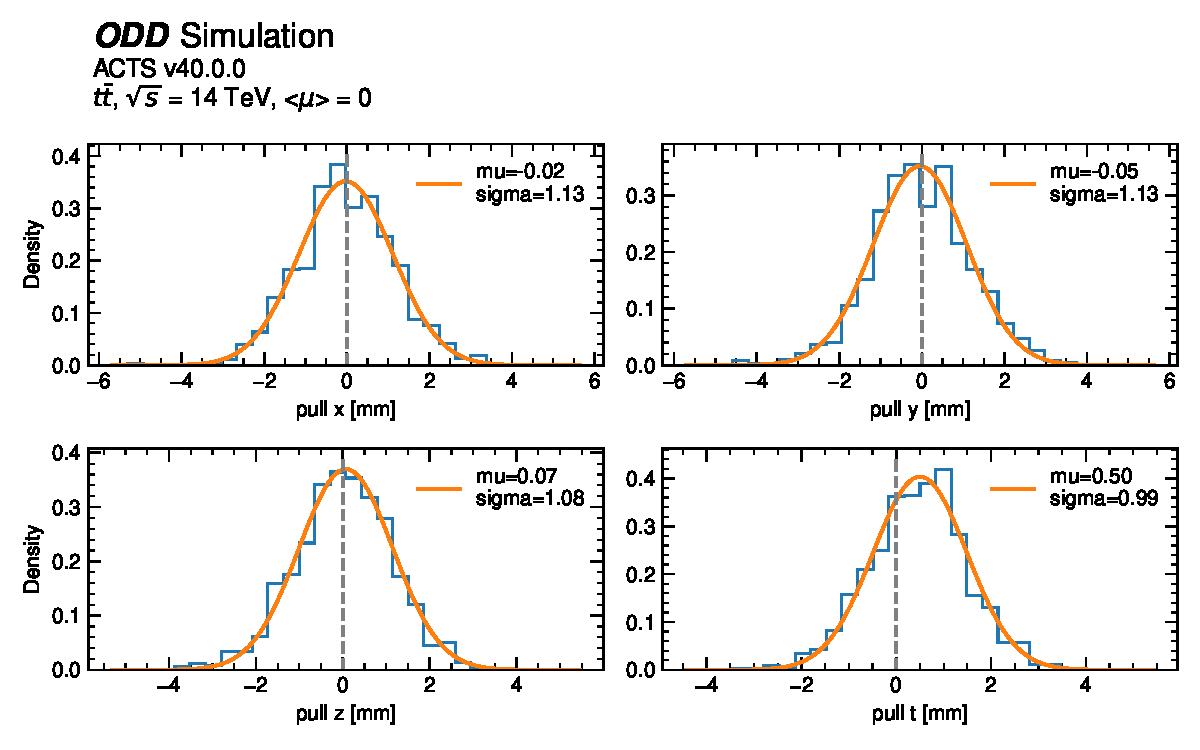
\includegraphics[width=1.0\textwidth]{parts/3_performance/11_acts-performance/figures/vertex_pull.pdf}
    \caption{}
    \label{fig:perf/odd/vertex-pull}
\end{figure}

\section{Computation time}

\begin{figure}[h]
    \centering
    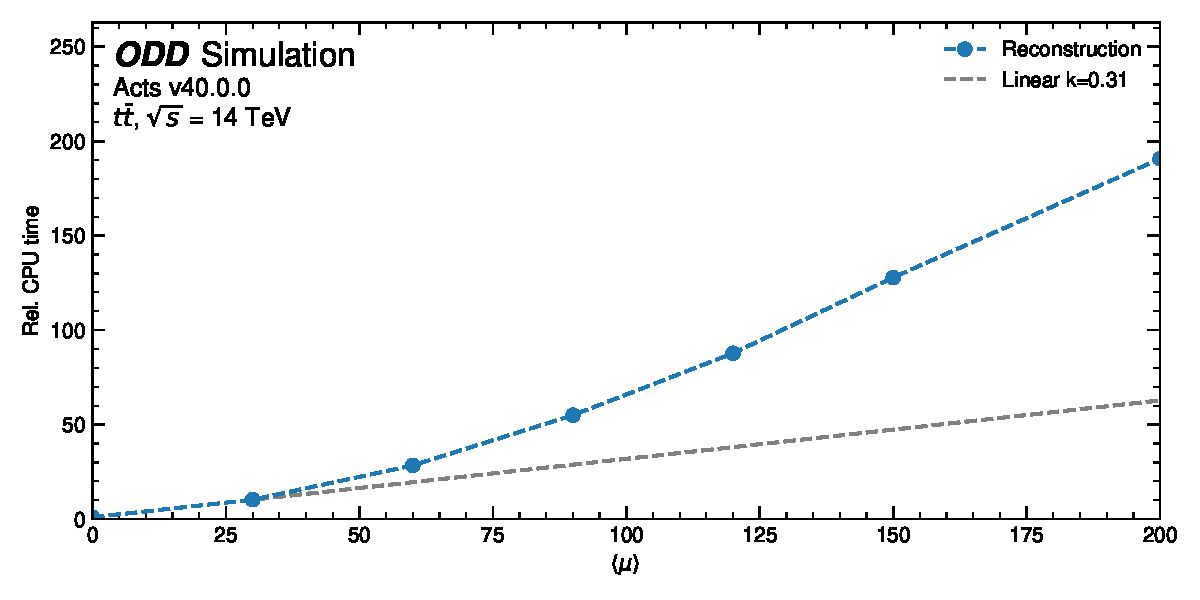
\includegraphics[width=1.0\textwidth]{parts/3_performance/11_acts-performance/figures/cpu_total_ttbar.pdf}
    \caption{}
    \label{fig:perf/odd/cpu-total-ttbar}
\end{figure}

\begin{figure}[h]
    \centering
    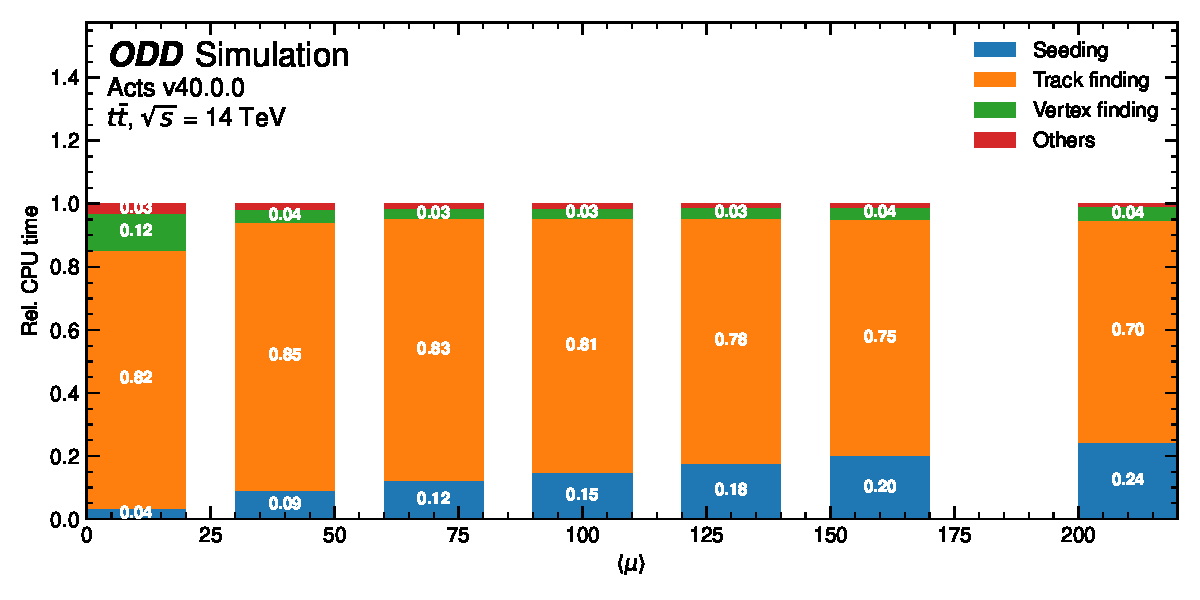
\includegraphics[width=1.0\textwidth]{parts/3_performance/11_acts-performance/figures/cpu_alg_ttbar.pdf}
    \caption{}
    \label{fig:perf/odd/cpu-alg-ttbar}
\end{figure}
